\section{Botnet, des codes malveillants organisés}.

A titre d'illustration, je vous propose de découvrir les botnets avec les travaux de David Batany.
Le Botnets font partis de ce que nous pourrions appelé des architectures techniques malveillantes. En effet, un Botnet en lui même est un code malveillant qui fonctionnement dans une architecture informatique complexe avec des mécanismes de pilotage, de stockage, de réplication et d'activation spécialisées. Un Botnet est peut être considéré comme un système d'arme utilisable pour des attaques.

%\newcommand{ \localpath}{../Contribs/david.batany@contribs.cyberdef/}
%\input{\localpath botnet.proxy.tex}


%Historique-motivations-Architecture_de_BOTNET

\subsection{Définition}
\par
Le terme \textbf{botnet}, contraction de l'anglais \textbf{robot+net}, se définit par l'ensemble des programmes, machines, serveurs connectés à internet ayant un ou plusieurs processus commun de communication.
Placé sous le contrôle d'un opérateur humain, appelé botmaster, le botnet recrute des machines en exploitant les vulnérabilités, failles, infections afin d'étendre son réseau à travers l'utilisation de canaux de Command and Control(C\&C).
\newline Avec l'IoT\footnote{Internet of Things}, et ses appareils connectés, le réseau s'étend de plus en plus au sein de notre société. L'actuelle faiblesse en terme de sécurité lié aux objets connectés représente une menace majeure et croissante dans notre environnement.
\head{Historique}
\par
Le concept, inventé en 1988 à l'université de Oulu en Finlande, fut développé à l'origine pour gérer les services associés au protocole IRC\footnote{Internet Relay Chat, un protocole de communication textuel}.
\newline
Le premier bot \g{<GM}> assistait ainsi l'utilisateur dans la gestion des connections IRC.
Cette gestion automatisée, permettant via un accès à distance, de contrôler et de réaliser des opérations a très vite montré un haut pouvoir malveillant.
\newline
En Mai 1999, Pretty Park, un malware de forme trojan horse se propageant sur le net permettait de voler les mots de passe.
\newline
Les premières dérives furent notamment l'affrontement de botnet IRC (\href{https://www.eggheads.org/}{Eggdrop} en décembre 1993, puis GTbot en avril 1998).
\head{Motivations liées à la menace botnet}
\begin{itemize}
	\item L'aspect lucratif représente l'intérêt majeur pour l'utilisateur de botnet. L'automatisation d'une tâche contrôlée à distance permettant de rapporter facilement des revenus (revente d'information, fraude au clic, spam), surtout si celle-ci est réalisée de manière anonyme(réseau TOR\footnote{The Onion Routing, un réseau d'anonymisation}).
	\item La motivation idéologique, comme par exemple, lors du conflit entre la Georgie et la Russie en 2008 ou de nombreux sites étatiques faisait l'objet de cyberattaques massives paralysaient les infrastructures.
	\item La motivation personnelle, à travers la vengeance ou le chantage, est également une finalité grâce notamment au caractère anonyme de l'attaque.
\end{itemize}


%Attaque-Architecture_de_BOTNET

\subsection{Les utilisations des Botnets}
On peut citer les attaques classiques utilisant des techniques de botnets:
\begin{itemize}
	\item Déni de service distribué (DDoS\footnote{Distributed Denial of Service}) ;
	\item DDoS contre paiement ;
	\item Cryptominage ;
	\item Récupération des identifiants;
	\item Exposition médiatique ou démonstration de force ;
	\item Dissimulation d’une autre attaque;
	\item Création d’un avantage concurrentiel ;
	\item Censure par attaque de serveurs;
	\item Vengeance par cryptolocker;
	\item Infrastructure d’anonymisation ;
	\item Recherche de vulnérabilités;
	\item Infrastructure d’anonymisation des communications;
	\item Contournement de mesures de limitation ou blocage ;
	\item Envoi de pourriels (Spam);
	\item Diffusion de codes malveillants;
	\item Exécution de codes malveillants sur les machines-zombies;
	\item Hébergement de codes malveillants ;
	\item Fraude aux clics ;
	\item Compromission d’accès ;
	\item Brute force hors-ligne;
	\item Brute force direct ...

\end{itemize}

%CycleDeVie-Architecture_de_BOTNET

\subsection{Cycle de vie d'une attaque:}
\par Pour la compréhension, il est nécessaire de comprendre les différentes étapes depuis l'infection jusqu'au fonctionnement complet du botnet.

\head{Infection de la machine}  \head{}
Cette première étape a généralement pour but de télécharger la charge virale sur un serveur.
Elle peut être initiée via les vecteurs suivants:
	 \begin{itemize}
		 \item Par spam (existence de spambot)
		 \item Exploitation de faille lié à la navigation sur un site web (malvertising\footnote{exploitation de pop-up publicitaires}, waterholing\footnote{ciblage de sites web fréquentés})
		 \item P2P
		 \item Spear phishing\footnote{hameçonnage ciblé pour récupérer données ou identifiants}
		 \item SMS, MMS
		 \item Bluetooth
		 \item TDS\footnote{Traffic Distribution Service, outil et service de redirection de trafic}
		 \item Exploit kits\footnote{plate-forme d'exploitation supporté par un site web permettant de tester une liste d'exploits}
	 \end{itemize}
	
\head{Activation}
Après téléchargement, l'installation du malware peut établir un premier contact avec le botnet (serveur dédié, servant-bot) ayant une fonctionnalité de C\&C.
Le téléchargement de \gls{gROOTKIT} d'installation ou de \gls{aDLL} complémentaire finalise la mise en place du botnet sur la machine infectée.	
	
\head{Mise à jour}
Les échanges permettent l'ajout de fonctionnalité, de configurations afin que le botnet puisse identifier et s'adapter à son environnement.
Il peut, par exemple, vouloir modifier son hash\footnote{signature numérique, ici on parle de signature virale} afin de conserver une certaine furtivité pour la continuité de l'attaque.

\head{Auto-protection}
La persistance et la dissimulation sont les facteurs clés de cette étape. L'installation de rootkit de protection, la modification du système, etc permettent de masquer l'action du botnet.
	
\head{Propagation}
Cette phase d'extension est à la fois locale par du scan et distante par diffusion virale (mail avec lien ou pièce jointe).
	
\head{Phase opérationnelle}
Cette dernière phase vise à accomplir les actions souhaitées de l'attaquant. 
Déclenchées, synchronisées ou persistantes ces attaques s'adaptent aux cibles désignées.Ordonné par le C\&C elles peuvent être activées ou mises en sommeil afin de ne pas attirer l'attention.




%Menace-Architecture_de_BOTNET

\subsection{Les type de menaces}
Les botnets représentent les outils de diffusion des attaques.
Cet outil permet aux cybercriminels de disposer d'un grand nombre de services développé dans un environnement collaboratif. Vendus sur le web, ils instrumentalisent l'attaque quelque soit le but recherché.
\newline \textbf{Liste des menaces possibles:}
\begin{itemize}
	\item Relayer du spam pour du commerce illégal ou pour de la manipulation d'information (par exemple des cours de bourse) 
  \item Réaliser des opérations d'hameçonnage 
  \item Identifier et infecter d’autres machines par diffusion de virus et de programmes malveillants (malwares) 
  \item Participer à des attaques groupées de déni de service (DDoS)
  \item Générer de façon abusive des clics sur un lien publicitaire au sein d’une page web (fraude au clic) 
  \item Capturer de l’information sur les machines compromises (vol puis revente d'information) ;
  \item Exploiter la puissance de calcul des machines ou effectuer des opérations de calcul distribué notamment pour cassage de mots de passe 
  \item Voler des sessions utilisateurs par credential stuffing ;
  \item Mener des opérations de commerce illicite en gérant l'accès à des sites de ventes de produits interdits ou de contrefaçons via des techniques de fast flux, simple ou double-flux ou RockPhish 
  \item Miner des cryptomonnaies, telles que le bitcoin1.
\end{itemize}

%Section-archi-aleatoire-Architecture_de_BOTNET

\newpage\subsection{Architecture aléatoire}

\upicture{\upath/Pictures/img-reseau_aleatoire}{Architecture aléatoire}{0.75}{}

%\begin{figure}[h]
%	\centering
%		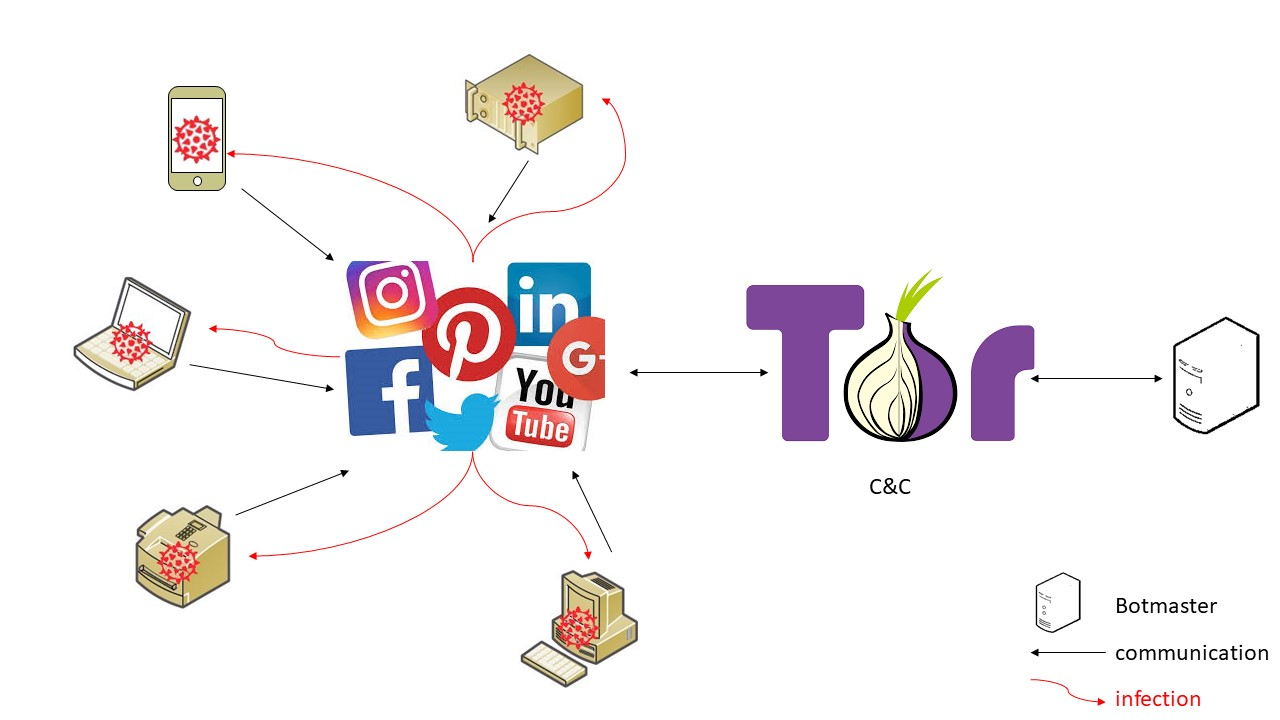
\includegraphics[width=0.75\textwidth]{reseau_aleatoire}
%	\label{fig:réseau_aléatoire}
%	\caption[Architecture aléatoire]{Architecture aléatoire}
%\end{figure}

\subsubsection{Définition}
Ce concept représente une variante de l'architecture centralisée et peut se retrouver dans une variété de malware connue sous le nom de RATs\footnote{Remote Access Trojan}.Ces chevaux de Troie fonctionnent sur un principe de client/serveur parfois mis en place avec des techniques de social engineering (exemple: un fichier d'installation récupéré sur un site douteux). Ils exécutent la partie client à l'insu de l'utilisateur pour se connecter au serveur.
\newline Cette architecture tire profit de l'exploitation de plate-formes existantes supportant le protocole HTTP comme Facebook, Twitter, Yahoo, Evernote, Google, etc. et de réseau permettant de camoufler les échanges comme TOR, Hornet, etc.

\subsubsection {Liste des protocoles utilisés par le botnet}
\begin{itemize}
	\item HTTP
	\item protocole propriétaire (exemple XMPP\footnote{Extensible Messaging and Presence Protocol de MSN Messenger})
	\item IRC
\end{itemize}

\subsubsection{Avantages}
\begin{itemize}
	\item Architecture déjà existante
	\item Réseau important en terme d'utilisateurs
	\item Utilisation des canaux existants (exemple: messagerie instantanée)
	\item utilisation des fonctionnalités du réseau (exemple :Le réseau anonymisation TOR)
	\item Difficulté de démanteler son propre réseau
\end{itemize}

\subsubsection{Inconvénients}
\begin{itemize}
	\item Vulnérabilité du botnet face aux mécanismes de défense
	\item Connexion en permanence
	\item bloqué par le filtrage de liens de la plate-forme
\end{itemize}

%--------------------------------------------------------------------
%ajouter un botnet
%glisser le .csv dans le dossier exemples de la section 2
%inclure la ligne \csvautotabular[respect all]{Section/2-Ssection/exemples/nom-du-botnet}
%--------------------------------------------------------------------


\subsubsection{exemples}


%\noindent
%\resizebox{\textwidth}{!}{
%\csvautotabular[respect all]{Section/2-Ssection/exemples/Cutwail.csv}
%}
%\resizebox{\textwidth}{!}{
%\csvautotabular[respect all]{Section/2-Ssection/exemples/Carna.csv}
%}




%Section-archi-centralise-Architecture_de_BOTNET


\subsection[Architecture  centralisée]{Architecture  centralisée}

%\begin{figure}[h]
%	\centering
%		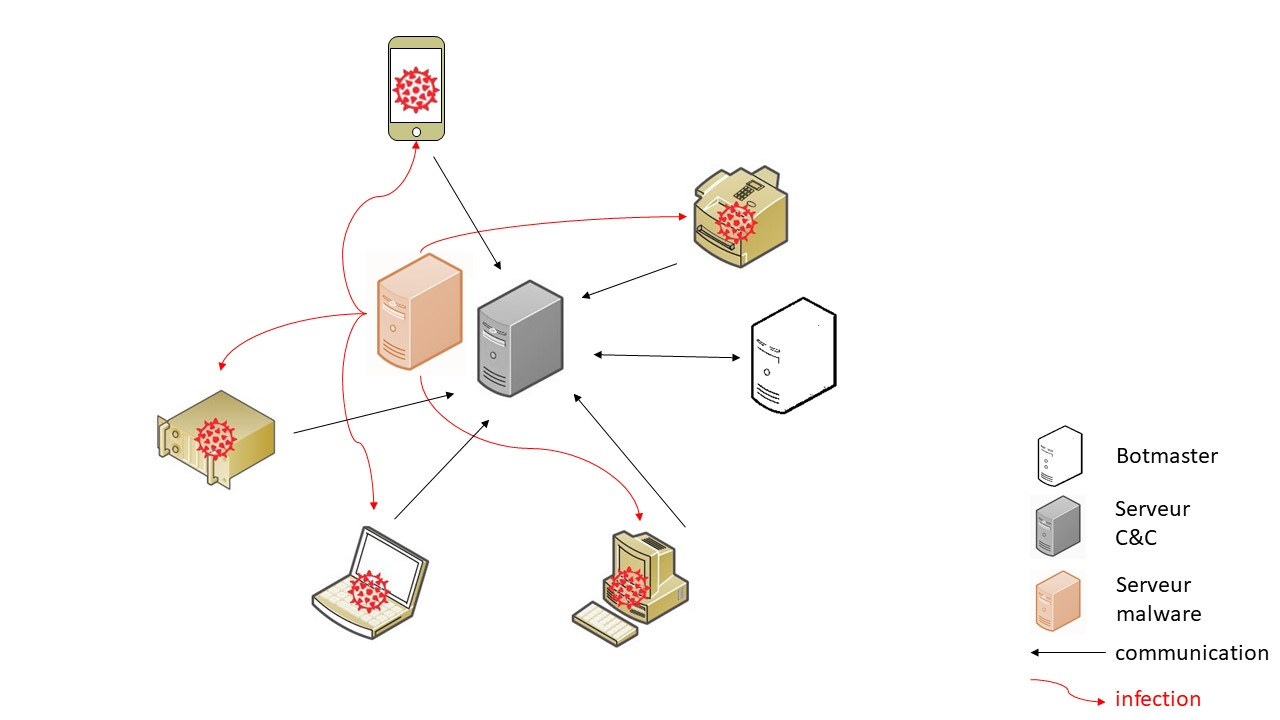
\includegraphics[width=0.75\textwidth]{archi_centralise}
%	\label{fig:archi_centralisée}
%	\caption[Architecture  centralisée]{Architecture  centralisée}
%\end{figure}


%\begin{figure}[h]
%	\centering
%		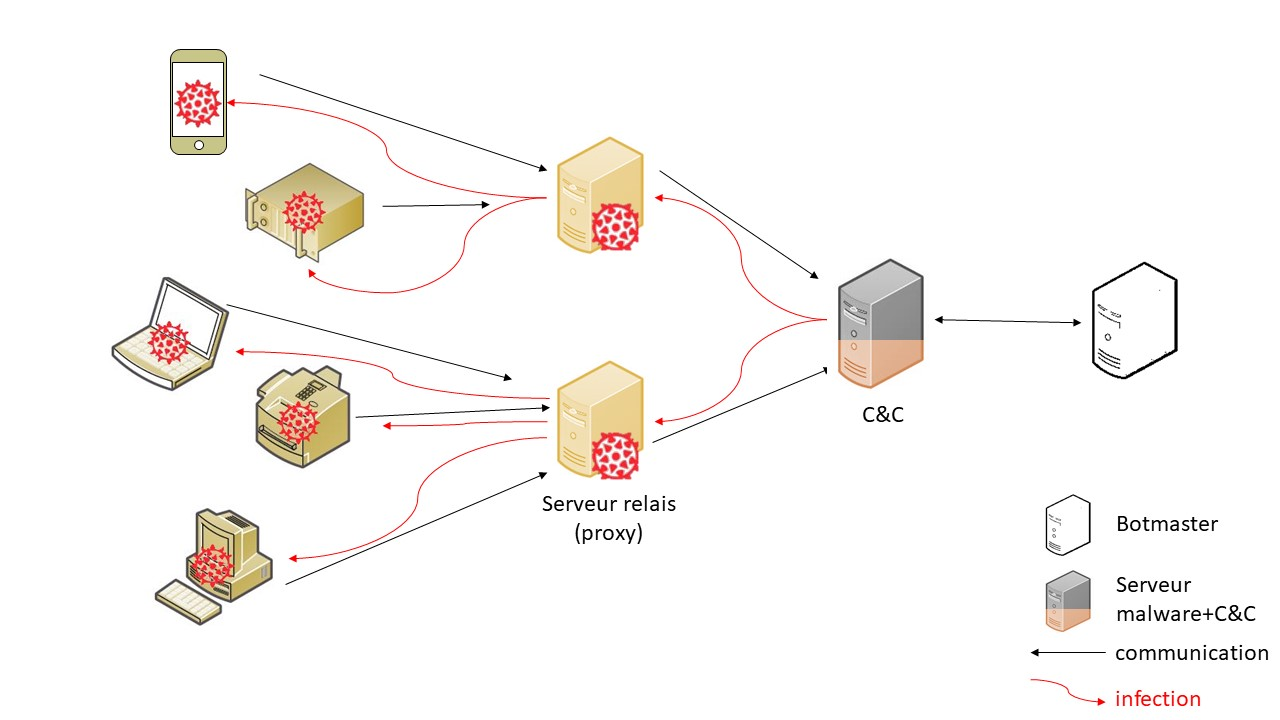
\includegraphics[width=0.75\textwidth]{archi_centralise_2}
%	\label{fig:Archi_centralisé_2}
%	
%	\caption[Architecture  centralisée répartie par utilisation d’une batterie de serveurs relais]{Architecture  centralisée répartie par utilisation d’une batterie de serveurs relais}
%\end{figure}

\subsubsection{Définition}
Un ou plusieurs nœud de communication permettent aux bots d'échanger des données via un canal de communication.
Les nœuds représentent un serveur ou serveur relais avec comme fonction le C\&C.

\subsubsection{Liste des protocoles utilisés par le botnet}
\begin{itemize}
	\item IRC\footnote{Internet Relay Chat}
	\item HTTP\footnote{HyperText Transfer Protocol}
	\item IRC modifié
\end{itemize}

\subsubsection{Avantages}
\begin{itemize}
	\item Architecture  centraliséee
	\item Simplicité de mise en oeuvre (mIRC, ...)
	\item Utilisation des canaux IRC (topics, messages) pour l’envoi des commandes vers les botsPerformance (non gourmant en bande passante)
	\item Connexions régulières entre les bots et le C\&C (non-permanente)
	\item Recherche des ordres dans des forums, avec des mots clés ou même dans des images (stéganographie)
\end{itemize}

\subsubsection{Inconvénients}
\begin{itemize}
	\item Vulnérabilité du botnet (serveur central)
	\item Connexion en permanence
	\item Facile à détecter (filtrage du flux IRC)
\end{itemize}

%--------------------------------------------------------------------
%ajouter un botnet
%glisser le .csv dans le dossier exemples de la section 2
%inclure la ligne \csvautotabular[respect all]{Section/2-Ssection/exemples/nom-du-botnet}
%--------------------------------------------------------------------


%\subsubsection{exemples}
%\noindent
%\resizebox{\textwidth}{!}{
%\csvautotabular[respect all]{Section/2-Ssection/exemples/BEBLOH.csv}
%}
%\noindent
%\resizebox{\textwidth}{!}{
%\csvautotabular[respect all]{Section/2-Ssection/exemples/BOBAX-KRAKEN.csv}




%Section-archi-decentralise-Architecture_de_BOTNET


\subsection{Architecture décentraliséee}

%\begin{figure}[h]
%	\centering
%		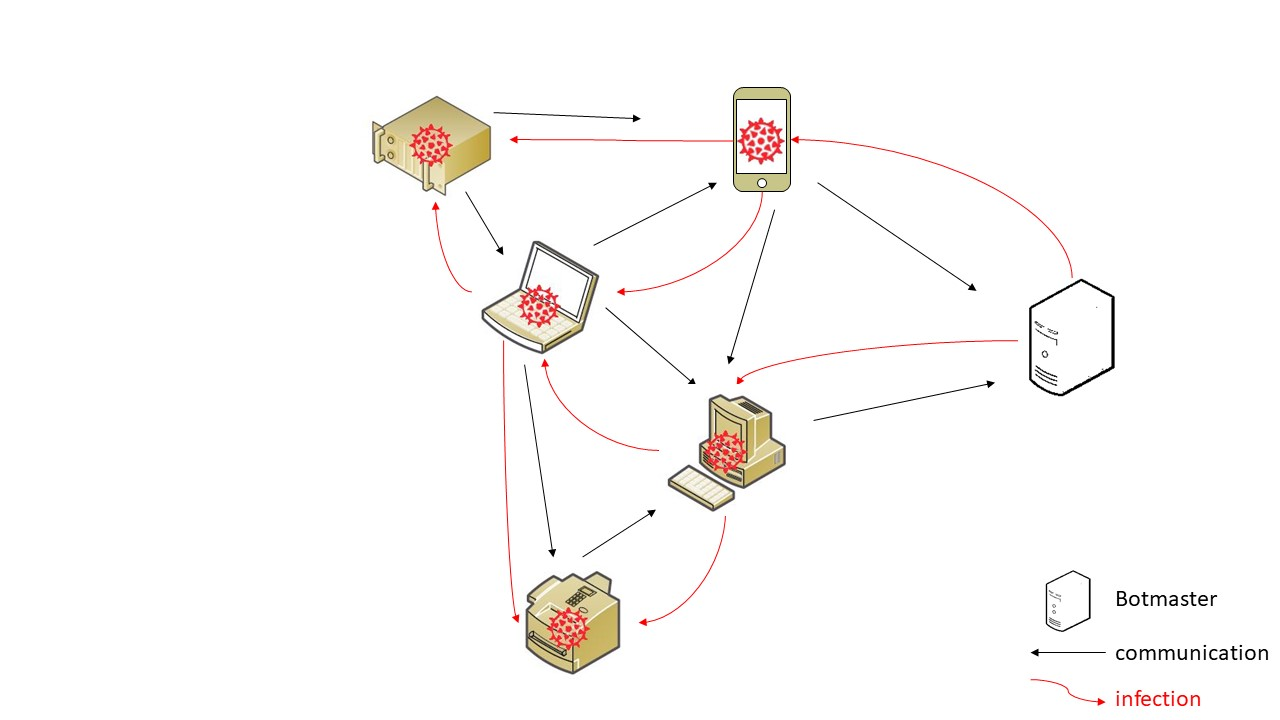
\includegraphics[width=0.75\textwidth]{P2P_non_structure}
%	\label{fig:P2P_non_structure}
%	\caption{P2P non structuré}
%\end{figure}
%\begin{figure}[h]
%	\centering
%		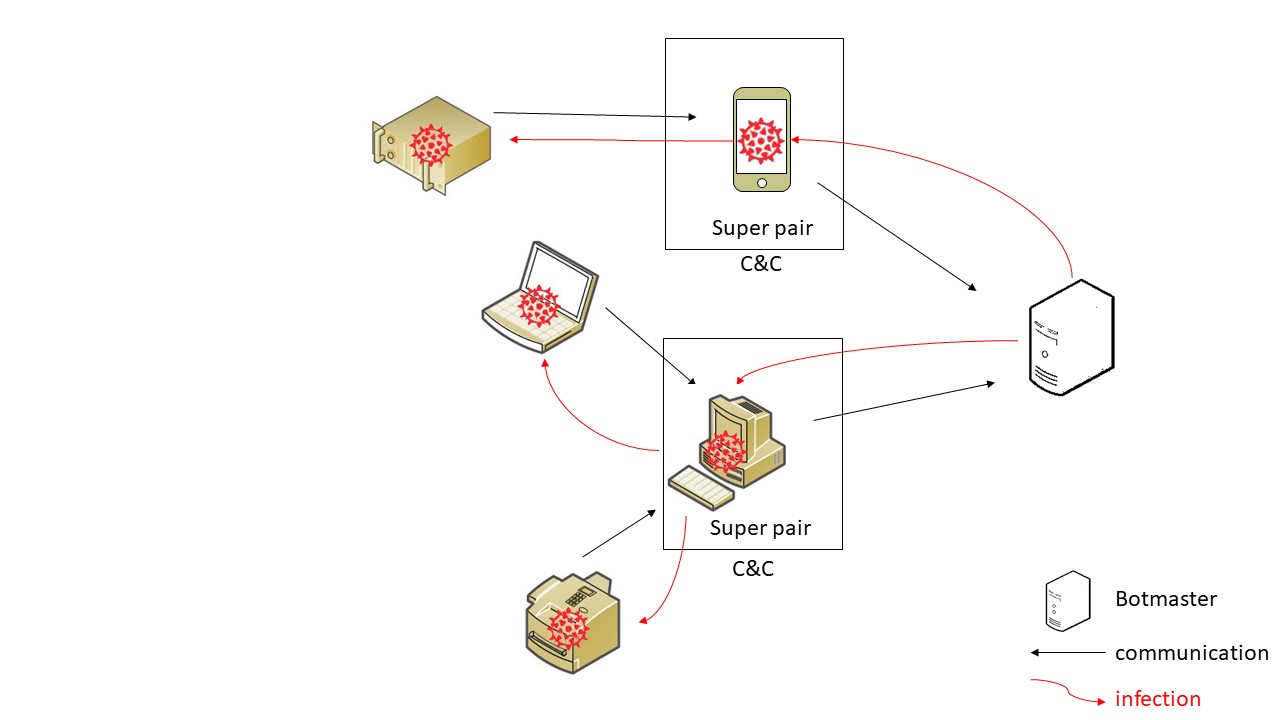
\includegraphics[width=0.75\textwidth]{P2P_avec_super_pairs}
%	\label{fig:P2P_avec_super_pairs}
%	\caption{P2P avec super-pairs}
%\end{figure}

\subsubsection{Définition}
\par En utilisant des réseaux peer-to-peer, on s’affranchit d'un point central de communication.Chaque bot, selon ses caractéristiques, apporte les ressources pour élaborer le système de C\&C.
Il existe plusieurs typologies de réseau overlay\footnote{réseau logique de recouvrement}:
\begin{itemize}
	\item \textbf{overlay P2P non-structuré} : les topologies sont aléatoires (loi de puissance, aléatoire uniforme,...)
  \item \textbf{overlay P2P par super-pairs} : tous les pairs du réseau ne sont pas égaux, certains d’entre eux étant automatiquement sélectionnés pour servir temporairement le rôle de serveur pour les recherches ou le contrôle du réseau (comme FastTrack ou Gnutella)
  \item \textbf{overlay P2P structuré} : une cartographie établissant le lien entre le contenu et son emplacement ; ce type de réseau implémente en général – mais pas systématiquement une table de hachage distribuée (DHT) ; on retrouve dans cette catégorie les protocoles P2P Chord, Tapestry et Kademlia (utilisé par le logiciel eMule).
\end{itemize}

\subsubsection{Liste des protocoles utilisés par le botnet}
\begin{itemize}
	\item TCP/IP
	\item UDP
\end{itemize}

\subsubsection{Avantages}
\begin{itemize}
	\item Architecture dé centraliséee
	\item Indépendant de l’architecture DNS
	\item difficile à repérer
	\item Connexions régulières entre les bots et le C\&C (non permanente)
	\item Le botmaster donne les informations comme un bot faisant partie du réseau
  \item L’information transite de voisin en voisin
	\item très difficile à neutraliser
\end{itemize}

\subsubsection{Inconvénients}
\begin{itemize}
	\item Pas de vision globale du réseau par un bot
	\item Connexion en permanence
	\item Facile à détecter (filtrage du flux IRC)
\end{itemize}

%--------------------------------------------------------------------
%ajouter un botnet
%glisser le .csv dans le dossier exemples de la section 2
%inclure la ligne \csvautotabular[respect all]{Section/2-Ssection/exemples/nom-du-botnet}
%--------------------------------------------------------------------

%\subsubsection{exemples}
%\noindent
%\resizebox{\textwidth}{!}{
%\csvautotabular[respect all]{Section/2-Ssection/exemples/Storm.csv}
%}
%\resizebox{\textwidth}{!}{
%\csvautotabular[respect all]{Section/2-Ssection/exemples/QAKBOT.csv}
%}

%Section-archi-hybride-Architecture_de_BOTNET
\subsection{Architecture hybride}

%\begin{figure}[h]
%	\centering
%		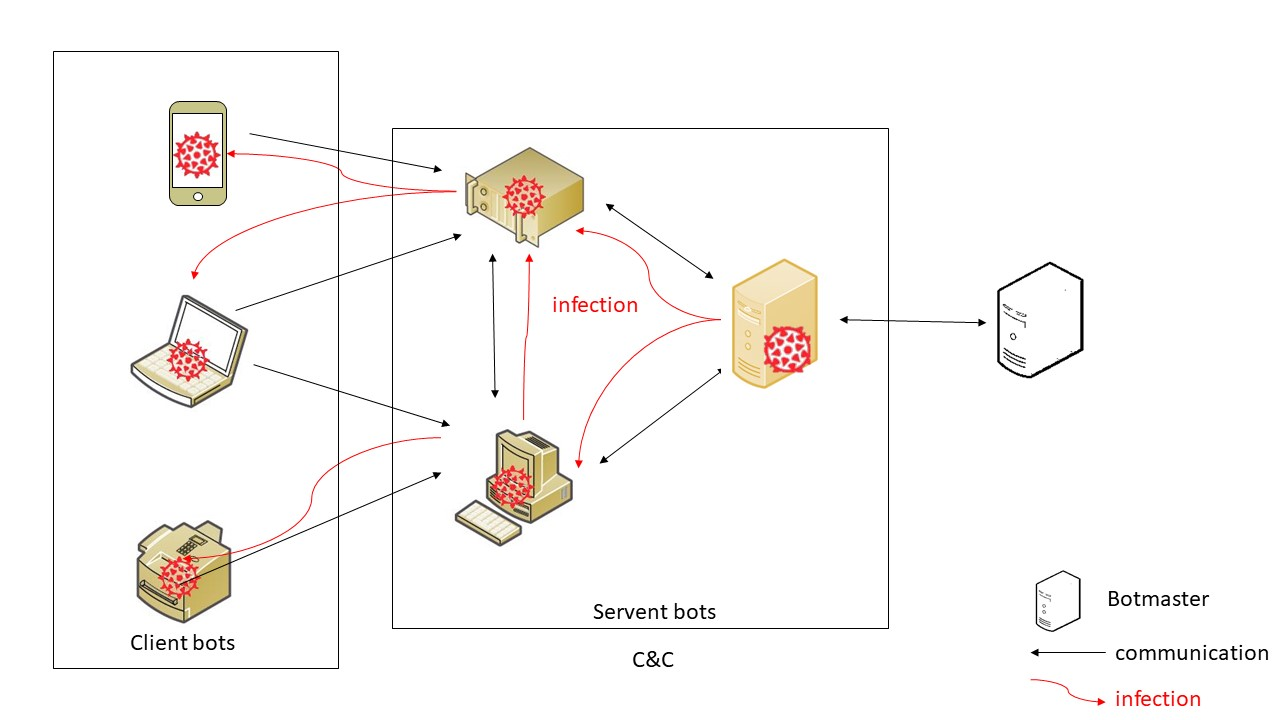
\includegraphics[width=0.75\textwidth]{structure_hybride_P2P}
%	\label{fig:structure_hybride_P2P}
%	\caption[Structure hybride P2P]{Structure hybride P2P}
%\end{figure}

\subsubsection{Définition}
Une architecture hybride intègre une solution de repli, comme à l'aide d'un DGA\footnote{Domain Generation Algorithm} ou de plusieurs niveaux successifs entre le P2P et le C\&C.Cette hiérarchie permet de masquer une partie des adresses IP utilisées afin de rendre plus complexe l'analyse du botnet.
L'association de bot clients et de bots servent\footnote{serv-\textbf{eur} et cli-\textbf{ent}} met en évidence l'organisation du réseau par le botmaster.
Ces niveaux intermédiaires permettent de solidifier l'architecture du réseau.

\subsubsection{Liste des protocoles utilisés par le botnet}
Reprenant les protocoles présentés dans les architectures précédentes, L'efficacité, la furtivité et la complexité des méthodes de communication ont pour objectif de nuire aux efforts de démantèlement.
Ainsi, les coopérations internationales entre acteurs institutionnels et
privés sont généralement nécessaires pour permettre de démanteler les botnets les plus sophistiqués.

\subsubsection{Avantages}
\begin{itemize}
	\item Nombre important de domaines
  \item masquage de l'adresse IP
\end{itemize}

\subsubsection{Iconvénients}
\begin{itemize}
	\item tributaire de la bande passante
\end{itemize}

%--------------------------------------------------------------------
%ajouter un botnet
%glisser le .csv dans le dossier exemples de la section 2
%inclure la ligne \csvautotabular[respect all]{Section/2-Ssection/exemples/nom-du-botnet}
%--------------------------------------------------------------------

\subsubsection{exemples}

%\noindent
%\resizebox{\textwidth}{!}{
%\csvautotabular[respect all]{Section/2-Ssection/exemples/Gameover-Zeus.csv}
%}
%\resizebox{\textwidth}{!}{
%\csvautotabular[respect all]{Section/2-Ssection/exemples/Mirai.csv}
%}

%$$$$$$$$$$$$$$$$$$$$$$$$$$$$$$$$$$$$$$$$$$$$$$$$

%Analyse-Architecture_de_BOTNET

\subsection{L'analyse} 
\subsubsection{L'analyse statique}
Réalisée en sandbox, sur une machine virtuelle ou une machine dédiée avec des outils pré-installés comme InetSim,FakeNet ou Mozzle, elle débute par une analyse statique pour identifier les éléments et la composition du malware.
L'examen du code et des fonctions appelées permettent d'évaluer les capacités du botnet.
\subsubsection{L'analyse dynamique} 
Cette étape est relativement utile pour la compréhension de la menace car elle présente la machine infectée sous plusieurs états à l'aide de snapshots\footnote{copie des données/modifications apportées à un système}.
Ces captures instantanées situent l'avancement de l'infection lors de l'attaque.
Il est souvent nécessaire en présence d'algorithme chiffré d'utiliser cette méthode pour désobfusquer le code et comprendre la structure du malware.


%Defense-et-blocage-Architecture_de_BOTNET

\subsection{La défense et le blocage}
Au même titre que la protection contre les malwares, les recommandations en terme de SSI\href{https://www.ssi.gouv.fr/administration/bonnes-pratiques/}{recommandations ANSSI}, applicables localement, doivent s'inscrire dans nos habitudes et augmentent ainsi la probabilité de bloquer l'étape initiale de l'infection (spam, navigation non-sécurisée,etc.).
\newline Les mises à jour logicielles et système sont essentielles pour bloquer l'exploitation de CVE\footnote{Common Vulnerabilities and Exposures} \href{https://www.cvedetails.com}{Common Vulnerabilities and Exposures}.
\newline Au niveau du FAI, les notifications en cas de connexions malveillantes et la surveillance des adresses IP sont un frein à l'extension du botnet.
\newline Enfin la détection d'un appel de fonctions anormal par l'antivirus, l'autorisation et l’identification des flux sortants par le firewall permettent le blocage de l'activité malveillante.
Les fonctionnalités recherchées de l'antivirus dans ce cadre sont un firewall bidirectionnel, une protection contre le phishing, la vérification de la certification, la lutte contre le tracking, la vérification du téléchargement, le blocage des pop-ups et pages WEB malveillantes,etc. 

%Demantelement-Architecture_de_BOTNET
\subsection{Le démantèlement}
Les méthodes de détection impliquent parfois des actions offensives visant à entraver le développement du botnet.
Il est cependant nécessaire d'avoir un support juridique et judiciaire pour mener à bien des actions adaptées au type et à la taille du botnet.
Celles-ci sont généralement menées en coopération avec les industriels (Microsoft,Level 3, Cisco,etc.) et la communauté scientifique.

%Detection-Architecture_de_BOTNET

\subsection{La détection}
Recherche d'anomalie, comparaison de signatures, pots-de-miel, toutes ces techniques basées sur l'activité du réseau reposent sur l'inspection des flux et des paquets.

\subsubsection{La détection passive}
L'identification et l'analyse passive des flux (adresses IP,port source et destination, étiquette MPLS\footnote{MultiProtocol Label Switching}, etc.) permettent de classifier les protocoles suspects et les serveurs de C\&C.
\newline BotFinder, par exemple, permet de décomposer un flux (durée moyenne des connexions, nombre d'octets transférés, etc.) et de le comparer à l'activité normale du réseau.
\newline L'observation des DNS\footnote{Domain Name Server} permet aussi d'identifier les domaines malveillants afin de caractériser le botnet suspecté.
BotGad, un système d'exploitation permettant d'analyser le trafic DNS sur un réseau local, utilise un algorithme basé sur l'apprentissage afin de définir la stratégie de groupe du botnet.
\newline EXPOSURE, un autre système d'exploitation déployé au sein de l'ISP\footnote{Internet Service Provider}, permet d'analyser à large échelle mais sur une durée de plusieurs mois le trafic DNS. Produisant une liste de domaines malveillants, il permet, par exemple, d'identifier un volume conséquent de requêtes pour un même domaine.
\newline Enfin le recours aux pots-de-miel et l'analyse des journaux d'activité sont les éléments de base d'une recherche d'activité liée aux botnets.
Suivant cette idée, le SIEM\footnote{Security Information and Event Management}, une solution de gestion de la sécurité, représente un outil précieux et novateur afin d'optimiser la veille du trafic et d'automatiser les processus de sécurité en cas de comportement anormal.

\subsubsection{La détection active}
Différentes techniques existent comme le sinkholing\footnote{également appelé serveur gouffre, gouffre Internet ou Blackhole DNS } redirigeant le trafic vers des serveurs afin de simuler le comportement du C\&C et de diminuer la puissance du réseau du botnet.
\newline L'infiltration, fonction de l'architecture du botnet, consiste à simuler le comportement d'un botnet contrôlé à l'aide de drones IRC ou de script afin de capturer le trafic et de remonter jusqu'au botmaster.
Le projet Pebbletrace reprend cette idée d’identification du botmaster en piégeant les équipements infectés avec une charge défensive afin de retourner le trafic contre le botnet.


%synthese
Les botnets font maintenant partie d'une économie souterraine sous forme de services payants.
Le harcèlement, le vol, les attaques par déni de service, etc figurent comme des produits de vente accessibles, moyennant finances, pour n'importe quel criminel.
\newline D'après l'ENISA\footnote{European Union Agency for Cybersecurity, anciennement European Network and Information Security Agency} les prix varient suivant la fiabilité, la durée et le type de service requis.
Par exemple une heure de DDoS est disponible pour 38\$.
Les différentes architectures permettent de mieux comprendre l'organisation du botnet et l'importance du C\&C.
\vspace{5mm}
\newline Les notions de veille technologique et de partage d'informations sur la menace sont essentielles du fait de l'implication du botnet dans les réseaux publiques et privés.
\newline Dans le cadre du renseignement lié aux menaces, les constructeurs de smartphone fournissent les informations (recherches, cibles des attaques, menaces associés aux mobiles, vulnérabilités des objets IoT) issues de leurs Threat Intelligence Center\footnote{Centre de renseignements liés aux menaces cyber}.
%ouverture
\vspace{5mm}
\newline Selon Nokia (\href{https://www.nokia.com/about-us/news/releases/2018/12/04/nokias-threat-intelligence-report-2019-warns-on-the-fast-growing-and-evolving-threat-of-malicious-software-targeting-internet-of-things-iot-devices/}{Nokia's Threat Intelligence Report}, l'activité des botnet sur l'IoT représente 78\% des événements de détection de malware en 2018.
\newline La menace omniprésente de ces objets connectés (santé, domotique, médias, électroménager,...) n'est aujourd'hui pas assez prise en considération par notre société de consommation.
Le manque de sécurité accrue de ces appareils faits apparaître ces objets connectés comme des acteurs potentiels constituant le réseau d'un botnet.
\newline L'arrivée prochaine de la 5G\footnote{prévisions en moyenne 100Mbit/S en download et 50 Mbit/s en upload} sera, dans ce domaine, un vecteur majeur pour la diffusion de l'infection du malware et le nombre d'attaques associés au botnet (exemple attaques DDoS).


%\begin{figure}[h!]
%\begin{center}
%	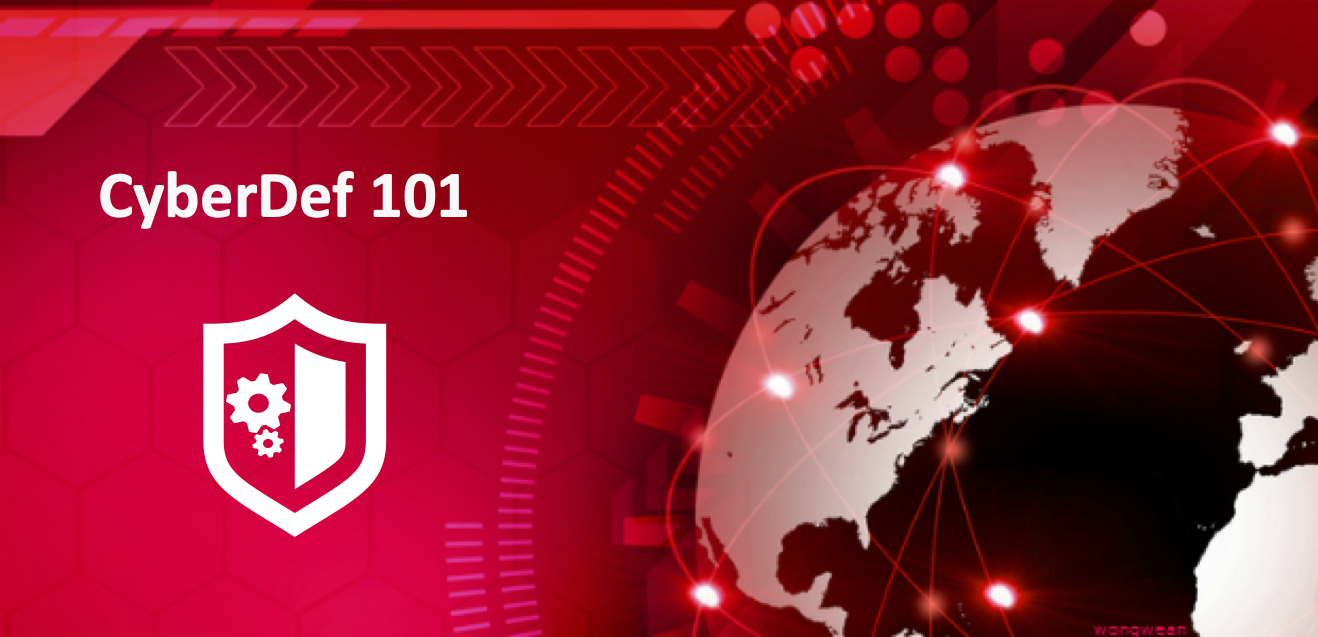
\includegraphics[width =0.6\textwidth, keepaspectratio]{coverback}
%	\caption{Figure 1}\label{mon image}
%	\end{center}
%\end{figure}